\section{Results} \label{sec:Results}
\noindent Using the implementation described the following results were obtained:
\subsection{Delay}
\noindent Through the use of the Quartus Signal Tap II Logic Analyser \cite{Signal_Tap}, it was possible to probe registers while the implementation was running on the FPGA in real time. As a result screen shots were taken documenting the achievements of the DRFM system. \\ \newline In Fig.~\ref{fig:delay}, the time delay functionality of the system can be seen. The the topmost value of the screen shot, \texttt{rdaddress}, is the address pointer to the RAM delay block. It can be seen that when the value \texttt{time\_delay} changes from 853 to 938 the \texttt{rdaddress} register changes from 1016 to 78 and increments by one for each subsequent clock cycle. It can be also seen that on the cycle after the \texttt{time\_delay} delay line changes, the \texttt{old\_time\_delay} line takes the \texttt{time\_delay}'s value. 
\begin{figure}[h!]
	\centering
	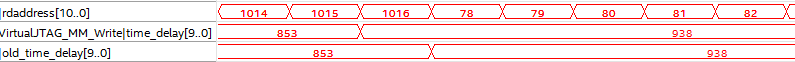
\includegraphics[width=\linewidth]{img/delay}
	\caption{Simulation Output Documenting a Time Delay}
	\label{fig:delay}
\end{figure}

\subsection{Frequency Shift}
	\noindent As already mentioned, the PWM module was used to output the waveforms through a GPIO pin on the FPGA development board. Therefore in order to obtain results about the frequency shift information, an Oscilloscope with FFT functionality was used to measure the frequency information of the PWM outputted signal. The results of the frequency shift were obtained by injecting $y(t)$ into SDRAM which can be expressed mathematically by
		\begin{equation}\footnotesize 
			y = cos(2\pi 10t) + cos(2\pi 20t)  + cos(2\pi 30t) + cos(2\pi 40t)+cos(2\pi 50t). \\
		\end{equation}
	\noindent It can be seen in Fig.~\ref{fig:1khz} that when the frequency shift on the UI was set to 1kHz, the output from the 8 bit PWM had a frequency of 1kHz. Furthermore, when the frequency was changed to 2kHz, the output also changed to 2kHz as can be seen in Fig.~\ref{fig:2khz}.
	\begin{figure}[h!]
	\centering
	\begin{subfigure}{0.48\linewidth}
		\centering
		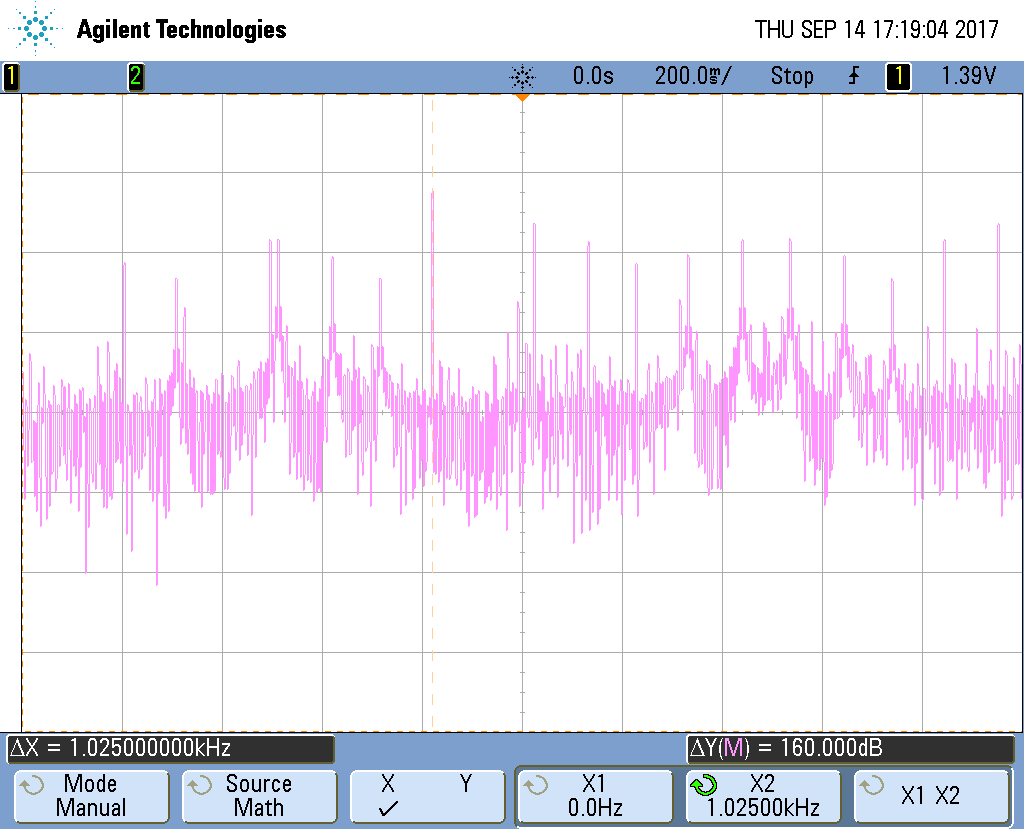
\includegraphics[width=.9\linewidth]{img/scope_3}
		\caption{Oscilloscope Print of a 1kHz frequency shift }
		\label{fig:1khz}
	\end{subfigure}%
	\begin{subfigure}{0.48\linewidth}
		\centering
		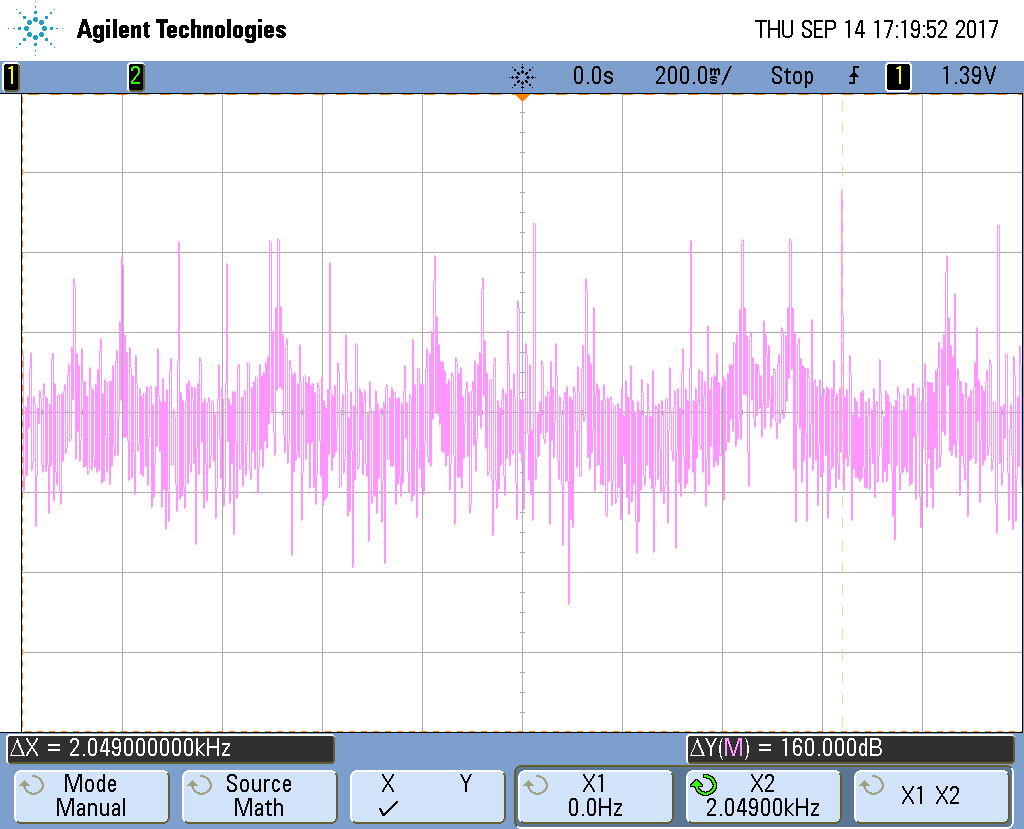
\includegraphics[width=.9\linewidth]{img/scope_4}
		\caption{Oscilloscope Print of a 2kHz frequency shift }
		\label{fig:2khz}
	\end{subfigure}
	\caption{Figures Showing the Measured Frequency Shift}
	\label{fig:2freq}
\end{figure}


\subsection{Amplitude Scaling}
	\noindent By using Quartus Signal Tap II Logic Analyser \cite{Signal_Tap}, it was possible to verify the amplitude scaling functionality of the DRFM system. In Fig.~\ref{fig:full_scale}, a full scale outputted sinusoid can be seen. In Fig.~\ref{fig:attentuated}, a fully attenuated sinusoid can be seen. This is as a result of the user sliding the amplitude scaling slider down to zero.
	\begin{figure}[h!]
	\centering
	\begin{subfigure}[b]{0.55\textwidth}
		\centering
		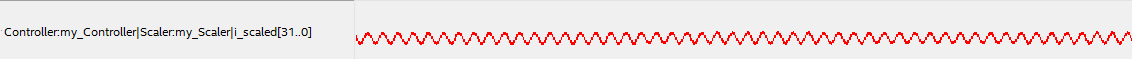
\includegraphics[width=.9\linewidth]{img/full_scale}
		\caption{Full Scale Sinusoid}
		\label{fig:full_scale}
	\end{subfigure}%


	\begin{subfigure}[b]{0.55\textwidth}
		\centering
		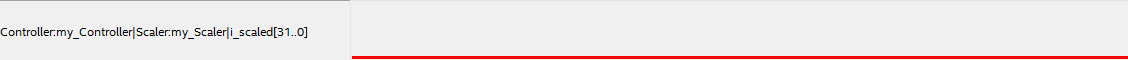
\includegraphics[width=.9\linewidth]{img/attenuated}
		\caption{Fully Attenuated Sinusoid}
		\label{fig:attentuated}
	\end{subfigure}
	\caption{Figures Showing the Measured Amplitude Scaling}
	\label{fig:amp}
\end{figure}
